\PassOptionsToPackage{unicode=true}{hyperref} % options for packages loaded elsewhere
\PassOptionsToPackage{hyphens}{url}
%
\documentclass[11pt,ignorenonframetext,]{beamer}
\usepackage{pgfpages}
\setbeamertemplate{caption}[numbered]
\setbeamertemplate{caption label separator}{: }
\setbeamercolor{caption name}{fg=normal text.fg}
\beamertemplatenavigationsymbolsempty
% Prevent slide breaks in the middle of a paragraph:
\widowpenalties 1 10000
\raggedbottom
\setbeamertemplate{part page}{
\centering
\begin{beamercolorbox}[sep=16pt,center]{part title}
  \usebeamerfont{part title}\insertpart\par
\end{beamercolorbox}
}
\setbeamertemplate{section page}{
\centering
\begin{beamercolorbox}[sep=12pt,center]{part title}
  \usebeamerfont{section title}\insertsection\par
\end{beamercolorbox}
}
\setbeamertemplate{subsection page}{
\centering
\begin{beamercolorbox}[sep=8pt,center]{part title}
  \usebeamerfont{subsection title}\insertsubsection\par
\end{beamercolorbox}
}
\AtBeginPart{
  \frame{\partpage}
}
\AtBeginSection{
  \ifbibliography
  \else
    \frame{\sectionpage}
  \fi
}
\AtBeginSubsection{
  \frame{\subsectionpage}
}
\usepackage{lmodern}
\usepackage{amssymb,amsmath}
\usepackage{ifxetex,ifluatex}
\usepackage{fixltx2e} % provides \textsubscript
\ifnum 0\ifxetex 1\fi\ifluatex 1\fi=0 % if pdftex
  \usepackage[T1]{fontenc}
  \usepackage[utf8]{inputenc}
  \usepackage{textcomp} % provides euro and other symbols
\else % if luatex or xelatex
  \usepackage{unicode-math}
  \defaultfontfeatures{Ligatures=TeX,Scale=MatchLowercase}
\fi
\usecolortheme{seahorse}
% use upquote if available, for straight quotes in verbatim environments
\IfFileExists{upquote.sty}{\usepackage{upquote}}{}
% use microtype if available
\IfFileExists{microtype.sty}{%
\usepackage[]{microtype}
\UseMicrotypeSet[protrusion]{basicmath} % disable protrusion for tt fonts
}{}
\IfFileExists{parskip.sty}{%
\usepackage{parskip}
}{% else
\setlength{\parindent}{0pt}
\setlength{\parskip}{6pt plus 2pt minus 1pt}
}
\usepackage{hyperref}
\hypersetup{
            pdftitle={Race, Class, and Transit Oriented Development},
            pdfauthor={Thelonious Goerz},
            pdfborder={0 0 0},
            breaklinks=true}
\urlstyle{same}  % don't use monospace font for urls
\newif\ifbibliography
\usepackage{graphicx,grffile}
\makeatletter
\def\maxwidth{\ifdim\Gin@nat@width>\linewidth\linewidth\else\Gin@nat@width\fi}
\def\maxheight{\ifdim\Gin@nat@height>\textheight\textheight\else\Gin@nat@height\fi}
\makeatother
% Scale images if necessary, so that they will not overflow the page
% margins by default, and it is still possible to overwrite the defaults
% using explicit options in \includegraphics[width, height, ...]{}
\setkeys{Gin}{width=\maxwidth,height=\maxheight,keepaspectratio}
\setlength{\emergencystretch}{3em}  % prevent overfull lines
\providecommand{\tightlist}{%
  \setlength{\itemsep}{0pt}\setlength{\parskip}{0pt}}
\setcounter{secnumdepth}{0}

% set default figure placement to htbp
\makeatletter
\def\fps@figure{htbp}
\makeatother


\title{Race, Class, and Transit Oriented Development}
\providecommand{\subtitle}[1]{}
\subtitle{\emph{Examining high-income demographic change after light rail transit}}
\author{Thelonious Goerz}
\providecommand{\institute}[1]{}
\institute{Dept. of Sociology\\
Johns Hopkins University\\
Center for Studies in Demography and Ecology}
\date{}

\begin{document}
\frame{\titlepage}

\begin{frame}{Outline}
\protect\hypertarget{outline}{}

\begin{itemize}
\tightlist
\item
  Background and prior research
\item
  Seattle case study
\item
  Methods and data
\item
  Descriptive and statistical results
\item
  Conclusion
\end{itemize}

\end{frame}

\begin{frame}{Motivation}
\protect\hypertarget{motivation}{}

\begin{itemize}
\tightlist
\item
  How and where people move have been a core questions in urban
  sociology and poverty research for years.
\item
  Moves and their associated neighborhood contexts are important for
  wellbeing, educational attainment, and development over the life
  course (Bergman et. al.~2020; Chetty et. al.~2016)
\item
  So it is important to understand the whole picture of mobility: Both
  high and low income mobility.
\end{itemize}

\textbf{But, does it makes sense to study the most vulnerable
populations?}

\end{frame}

\begin{frame}{Motivation}
\protect\hypertarget{motivation-1}{}

\textbf{Yes and No.}

\begin{itemize}
\tightlist
\item
  I argue an asymmetric focus on studying the movement patterns of
  low-income residents in changing neighborhoods has left open
  theoretical and empirical gaps for researchers.

  \begin{itemize}
  \tightlist
  \item
    We know little about the moves of high income individuals and
    households.
  \item
    Often elite wealthy individuals have more power and sway over
    government and economic processes (Gilens and Page 2014).
  \end{itemize}
\end{itemize}

\end{frame}

\begin{frame}{Background: Theory}
\protect\hypertarget{background-theory}{}

\begin{itemize}
\tightlist
\item
  Social scientists are interested in the effects of gentrification on
  urban demographic patterns.

  \begin{itemize}
  \tightlist
  \item
    In recent years, it has been linked to major urban re-investment
    projects, such as Light Rail Transit.
  \item
    So, transit is a good proxy for gentrification, neighborhood change,
    and associated ideas.
  \end{itemize}
\end{itemize}

\textbf{Why does studying transit matter?}

\end{frame}

\begin{frame}{Background: Theory}
\protect\hypertarget{background-theory-1}{}

\textbf{Seattle and many other cities are increasingly turning to Light
Rail Transit (LRT) as a way to manage growth, promote green travel
initiatives, and reduce congestion.}

\begin{itemize}
\tightlist
\item
  Manage the tech boom in WA.
\item
  Significant in-migration.
\item
  Population growth.
\end{itemize}

\end{frame}

\begin{frame}{The Present Study}
\protect\hypertarget{the-present-study}{}

\textbf{In Seattle:}

\begin{itemize}
\tightlist
\item
  The Link Light Rail has been in development since 1996 when it was
  approved.

  \begin{itemize}
  \tightlist
  \item
    Construction began in 2003 and a majority of stations opened in
    2009.
  \item
    As of 2021 there are 14 stations.
  \item
    There are currently north and south expansions in development to
    2036.
  \end{itemize}
\end{itemize}

\textbf{As a consequence:}

\begin{itemize}
\tightlist
\item
  There are puzzling trends going on.

  \begin{itemize}
  \tightlist
  \item
    Hess (2020) finds dramatic increases in non-Hispanic White residents
    after LRT in Seattle.
  \item
    Declines in Asian and Hispanic residents after LRT.
  \end{itemize}
\end{itemize}

\textbf{How is this happening?}

\end{frame}

\begin{frame}{Background: Income and mobility}
\protect\hypertarget{background-income-and-mobility}{}

\textbf{Conventional wisdom suggests that neighborhoods change through
low-income displacement.}

\begin{itemize}
\tightlist
\item
  But, low-income residents are often much less mobile than
  middle-income and higher-income residents (Freeman 2005).
\item
  However, there is evidence to suggest that middle and upper income
  residents are far more mobile:

  \begin{itemize}
  \tightlist
  \item
    Ding et al. (2016): Increases in high credit score individuals'
    mobility in gentrified neighborhoods.
  \item
    Bartholemew and Ewing (2017): Disamenity effect in neighborhoods
    with urban development, homeowners moving out.
  \item
    Martin and Beck (2011): Higher status non-homeowners may be moving
    out of gentrified neighborhoods.
  \end{itemize}
\end{itemize}

\end{frame}

\begin{frame}{The Present Study}
\protect\hypertarget{the-present-study-1}{}

\begin{itemize}
\tightlist
\item
  The demographic trends in Seattle are not consistent with patterns of
  socioeconomic mobility in changing neighborhoods.

  \begin{itemize}
  \tightlist
  \item
    Often low-income groups are declining.
  \item
    But, statistically these groups are not as mobile.
  \end{itemize}
\end{itemize}

\textbf{Where is this demographic change happening on average?}

\end{frame}

\begin{frame}{Hypothesis}
\protect\hypertarget{hypothesis}{}

\begin{itemize}
\tightlist
\item
  \textbf{This study argues that middle and high income groups are the
  primary forces shifting neighborhood racial composition in LRT
  neighborhoods because of their capacity to move.}
\end{itemize}

\end{frame}

\begin{frame}{Data}
\protect\hypertarget{data}{}

\begin{itemize}
\tightlist
\item
  Time series data for 135 census tracts (Seattle, N = 540) and 24 LRT
  treated tracts {[}1990-2015{]}:

  \begin{itemize}
  \tightlist
  \item
    Income (by race), demographic variables, and controls.
  \item
    American Community Survey, Decennial Census Long Form, Hess (2020).
  \end{itemize}
\end{itemize}

\end{frame}

\begin{frame}[fragile]{Data: A note on working with the ACS}
\protect\hypertarget{data-a-note-on-working-with-the-acs}{}

\begin{itemize}
\tightlist
\item
  I assemble this panel dataset between 1990-2015 at 4 time points.

  \begin{itemize}
  \tightlist
  \item
    The 1990 and 2000 are census long form data that are geographically
    linked to the 2010 re-draw of census tracts.

    \begin{itemize}
    \tightlist
    \item
      This is accomplished using the IPUMS geographic crosswalk
      files.\footnote<.->{More info here:
        \url{https://www.nhgis.org/geographic-crosswalks}}
      \footnote<.->{I am happy to discuss this in more depth too if it
        is of interest to the team.}
    \end{itemize}
  \end{itemize}
\item
  I create income quintiles by matching the income bins in the ACS and
  Census data at time t to the cutoffs for each quintile in that year.

  \begin{itemize}
  \tightlist
  \item
    This has some issues, given there is error in the cutoffs.

    \begin{itemize}
    \tightlist
    \item
      Thankfully in this case the error is at most \$5,000.
    \end{itemize}
  \item
    The upper tail of the distribution is unknown so we have very little
    idea how much error there is.
  \end{itemize}
\item
  Data after 2009 can be accessed easily with the \texttt{tidycensus}
  package in R. This has excellent support and needs an API
  key!\footnote<.->{So get one if you need.}
\end{itemize}

\end{frame}

\begin{frame}{Methods}
\protect\hypertarget{methods}{}

\begin{itemize}
\tightlist
\item
  Difference in difference (DID) (comparative counterfactual design)
\item
  DID is a quasi-experimental research design borrowed from
  econometrics, that useses the assumption of ``parallel pre-treatement
  trends'' as an identification strategy for a causal effect.

  \begin{itemize}
  \tightlist
  \item
    This means that we find some panel data where there is a pre and
    post treatment stage, and compare pre-treatment states of both
    treatment and control groups.

    \begin{itemize}
    \tightlist
    \item
      If they are the same, we can assume that the post-treatment
      difference\footnote<.->{Here is where the name comes in.} is the
      effect of the treatment on the outcome.
    \end{itemize}
  \item
    The limitations and threats to identifcation are many, especially in
    this case.
  \end{itemize}
\end{itemize}

\end{frame}

\begin{frame}{Methods}
\protect\hypertarget{methods-1}{}

\begin{itemize}
\tightlist
\item
  To specify the model, I use robust standard errors clustered at the
  tract level and formulate the model in a maximum likelihood regression
  framework.
\item
  I specify the following model with the functional form:
\end{itemize}

\[
\begin{aligned}
  Y_{it} &= \alpha_i + \gamma_{t} + X_{it} +\beta{\delta_{1990}} + \beta{\delta_{2010}} + \beta{\delta_{2015}} + \epsilon_{it} \\
  \epsilon &\sim N(\mu,\sigma^2)
\end{aligned}
\]

\begin{itemize}
\tightlist
\item
  Where, Y is the percent of a racial group in a census tract at time t
  and in the treatment group i, alpha is a group fixed effect and gamma
  is a time fixed effect, and X is a matrix of control variables for the
  1980 composition and others. The deltas are interactions coefficients
  that correspond to pre-trend (1990), a reference category (2000), and
  a post-construction effect (2010) and a post link opening (2015)
  effect.
\end{itemize}

\end{frame}

\begin{frame}{Summary Statistics}
\protect\hypertarget{summary-statistics}{}

\begin{table}[!htbp] \centering 
  \caption{Pooled Cross-Sectional Pre-Treatment Summary Statistics (2000)} 
  \label{} 
\begin{tabular}{@{\extracolsep{5pt}}lccccc} 
\\[-1.8ex]\hline 
\hline \\[-1.8ex] 
Statistic & \multicolumn{1}{c}{N} & \multicolumn{1}{c}{Mean} & \multicolumn{1}{c}{St. Dev.} & \multicolumn{1}{c}{Min} & \multicolumn{1}{c}{Max} \\ 
\hline \\[-1.8ex] 
Percent White & 135 & 67.000 & 23.000 & 9.100 & 94.000 \\ 
Percent Black & 135 & 8.300 & 10.000 & 0.000 & 50.000 \\ 
Percent Asian & 135 & 13.000 & 13.000 & 0.880 & 58.000 \\ 
Percent Hispanic & 135 & 5.500 & 4.200 & 1.000 & 37.000 \\ 
Percent Q1 & 135 & 20.000 & 12.000 & 4.500 & 71.000 \\ 
Percent Q2 & 135 & 18.000 & 5.400 & 6.000 & 37.000 \\ 
Percent Q3 & 135 & 16.000 & 3.900 & 4.200 & 27.000 \\ 
Percent Q4 & 135 & 19.000 & 4.700 & 3.300 & 28.000 \\ 
Percent Q5 & 135 & 27.000 & 13.000 & 2.400 & 66.000 \\ 
\hline \\[-1.8ex] 
\end{tabular} 
\end{table}

\end{frame}

\begin{frame}{Summary Statistics}
\protect\hypertarget{summary-statistics-1}{}

\begin{table}[!htbp] \centering 
  \caption{Pooled Cross-Sectional Post-Treatment Summary Statistics (2015)} 
  \label{} 
\begin{tabular}{@{\extracolsep{5pt}}lccccc} 
\\[-1.8ex]\hline 
\hline \\[-1.8ex] 
Statistic & \multicolumn{1}{c}{N} & \multicolumn{1}{c}{Mean} & \multicolumn{1}{c}{St. Dev.} & \multicolumn{1}{c}{Min} & \multicolumn{1}{c}{Max} \\ 
\hline \\[-1.8ex] 
Percent White & 135 & 65.000 & 21.000 & 5.900 & 92.000 \\ 
Percent Black & 135 & 7.500 & 8.900 & 0.000 & 44.000 \\ 
Percent Asian & 135 & 14.000 & 12.000 & 2.400 & 63.000 \\ 
Percent Hispanic & 135 & 6.700 & 5.400 & 1.100 & 41.000 \\ 
Percent Q1 & 135 & 19.000 & 12.000 & 2.500 & 67.000 \\ 
Percent Q2 & 135 & 15.000 & 5.000 & 4.300 & 31.000 \\ 
Percent Q3 & 135 & 19.000 & 5.300 & 6.800 & 33.000 \\ 
Percent Q4 & 135 & 21.000 & 5.900 & 4.000 & 35.000 \\ 
Percent Q5 & 135 & 26.000 & 13.000 & 1.000 & 63.000 \\ 
\hline \\[-1.8ex] 
\end{tabular} 
\end{table}

\end{frame}

\begin{frame}{Summary Statistics: Treatment}
\protect\hypertarget{summary-statistics-treatment}{}

\begin{table}[!htbp] \centering 
  \caption{Treatment Group Cross-Sectional Pre-Treatment Summary Statistics (2000)} 
  \label{} 
\begin{tabular}{@{\extracolsep{5pt}}lccccc} 
\\[-1.8ex]\hline 
\hline \\[-1.8ex] 
Statistic & \multicolumn{1}{c}{N} & \multicolumn{1}{c}{Mean} & \multicolumn{1}{c}{St. Dev.} & \multicolumn{1}{c}{Min} & \multicolumn{1}{c}{Max} \\ 
\hline \\[-1.8ex] 
Percent White & 24 & 45.000 & 26.000 & 9.100 & 78.000 \\ 
Percent Black & 24 & 17.000 & 9.500 & 2.800 & 33.000 \\ 
Percent Asian & 24 & 24.000 & 18.000 & 5.000 & 58.000 \\ 
Percent Hispanic & 24 & 6.900 & 3.000 & 1.900 & 15.000 \\ 
Percent Q1 & 24 & 35.000 & 14.000 & 19.000 & 71.000 \\ 
Percent Q2 & 24 & 21.000 & 6.600 & 11.000 & 37.000 \\ 
Percent Q3 & 24 & 14.000 & 5.300 & 4.200 & 21.000 \\ 
Percent Q4 & 24 & 15.000 & 5.200 & 3.300 & 24.000 \\ 
Percent Q5 & 24 & 15.000 & 8.400 & 2.400 & 37.000 \\ 
\hline \\[-1.8ex] 
\end{tabular} 
\end{table}

\end{frame}

\begin{frame}{Summary Statistics: Treatment}
\protect\hypertarget{summary-statistics-treatment-1}{}

\begin{table}[!htbp] \centering 
  \caption{Treatment Group Cross-Sectional Post-Treatment Summary Statistics (2015)} 
  \label{} 
\begin{tabular}{@{\extracolsep{5pt}}lccccc} 
\\[-1.8ex]\hline 
\hline \\[-1.8ex] 
Statistic & \multicolumn{1}{c}{N} & \multicolumn{1}{c}{Mean} & \multicolumn{1}{c}{St. Dev.} & \multicolumn{1}{c}{Min} & \multicolumn{1}{c}{Max} \\ 
\hline \\[-1.8ex] 
Percent White & 24 & 48.000 & 21.000 & 12.000 & 75.000 \\ 
Percent Black & 24 & 14.000 & 10.000 & 2.900 & 35.000 \\ 
Percent Asian & 24 & 23.000 & 13.000 & 8.700 & 54.000 \\ 
Percent Hispanic & 24 & 8.000 & 5.100 & 2.700 & 25.000 \\ 
Percent Q1 & 24 & 30.000 & 10.000 & 14.000 & 49.000 \\ 
Percent Q2 & 24 & 17.000 & 5.300 & 7.600 & 31.000 \\ 
Percent Q3 & 24 & 18.000 & 4.900 & 8.300 & 26.000 \\ 
Percent Q4 & 24 & 18.000 & 4.900 & 9.000 & 25.000 \\ 
Percent Q5 & 24 & 17.000 & 7.700 & 5.500 & 36.000 \\ 
\hline \\[-1.8ex] 
\end{tabular} 
\end{table}

\end{frame}

\begin{frame}{Statistical Analysis: DID of racial composition}
\protect\hypertarget{statistical-analysis-did-of-racial-composition}{}

\begin{figure}
\centering
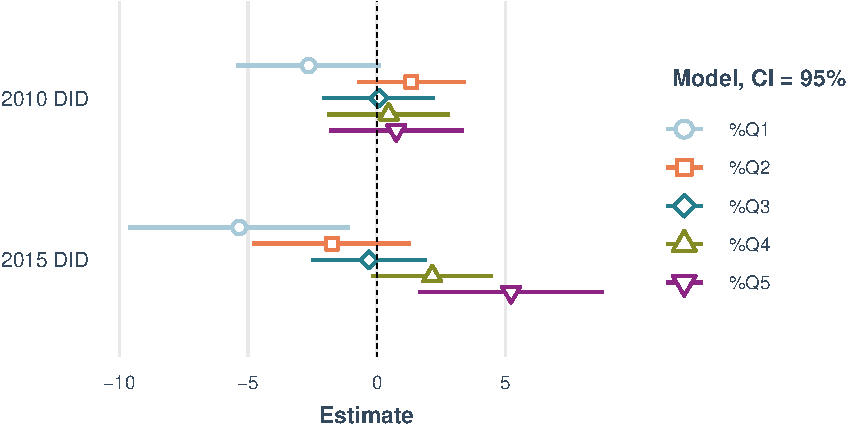
\includegraphics{csde_talk_files/figure-beamer/unnamed-chunk-11-1.pdf}
\caption{DID estimates of LRT effect on racial group percent}
\end{figure}

\end{frame}

\begin{frame}{Statistical Analysis: DID for income composition}
\protect\hypertarget{statistical-analysis-did-for-income-composition}{}

\begin{figure}
\centering
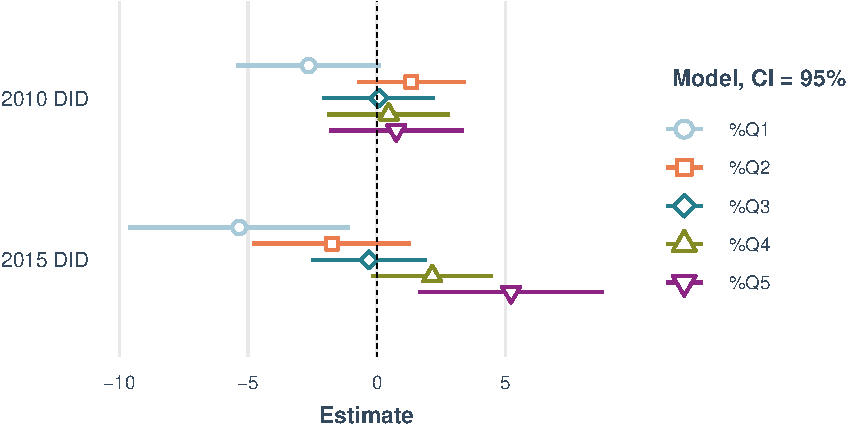
\includegraphics{csde_talk_files/figure-beamer/unnamed-chunk-13-1.pdf}
\caption{DID estimates of LRT effect on income quintile percent}
\end{figure}

\end{frame}

\begin{frame}{Conclusions}
\protect\hypertarget{conclusions}{}

\begin{itemize}
\tightlist
\item
  5 years after LRT, neighborhoods experience dramatic increases in
  white residents, and declining or stagnant non-white groups.
\item
  5 years after LRT, there is shift in the income distribution tending
  toward the highest quintile earners.\\
\item
  This suggests that income is an important factor in how demographics
  in Seattle are changing.
\item
  Income patterns are consistent with my hypothesis that dramatic shifts
  in income could be moving the composition.
\item
  Income does vary by racial group too. \#\# Edit
\end{itemize}

\end{frame}

\begin{frame}{Limitations}
\protect\hypertarget{limitations}{}

\begin{itemize}
\tightlist
\item
  The ACS and census report compositional estimates so understanding how
  distribution changes translate to in and out migration flows is
  tricky.
\item
  Prediction of Black racial and economic trends can be subject to a lot
  of uncertainty.\footnote<.->{Data and full analysis provided on
    request. Email:
    \href{mailto:tgoerz1@jh.edu}{\nolinkurl{tgoerz1@jh.edu}}}

  \begin{itemize}
  \tightlist
  \item
    Small counts in ACS sample.
  \item
    Low levels of Black population overall in Seattle.
  \end{itemize}
\item
  DID modeling assumptions may not be met in this case.\footnote<.->{Parallel
    trends and endogeneity are issues. I am happy to discuss these
    though.}
\end{itemize}

\end{frame}

\begin{frame}[fragile]{Future Directions}
\protect\hypertarget{future-directions}{}

\begin{itemize}
\tightlist
\item
  Examine LRT impact on just new in-movers using the ACS data.
\item
  Look at the differences in compositions between people who moved from
  the same county and those who are moving from out-of-county.
\item
  Look at the longer-term effect of LRT with the new 2020 ACS data.
\item
  Full models and analyses are on my github \texttt{theloniousgoerz}
  free and open to the public.

  \begin{itemize}
  \tightlist
  \item
    If you have questions about software or data let me know.
  \end{itemize}
\end{itemize}

\end{frame}

\begin{frame}{References}
\protect\hypertarget{references}{}

\fontsize{7pt}{7.2}\selectfont

Bartholomew, Keith, and Reid Ewing. 2011. ``Hedonic Price Effects of
Pedestrian- and Transit-Oriented Development.'' Journal of Planning
Literature 26(1):18--34. doi: 10.1177/0885412210386540.

Bergman, Peter, Raj Chetty, Stefanie DeLuca, Nathaniel Hendren, Lawrence
F. Katz, and Christopher Palmer. 2019. Creating Moves to Opportunity:
Experimental Evidence on Barriers to Neighborhood Choice. w26164.
National Bureau of Economic Research.

Bertrand, Marianne, Esther Duflo, and Sendhil Mullainathan. 2003. ``HOW
MUCH SHOULD WE TRUST DIFFERENCES-IN-DIFFERENCES ESTIMATES?'' 32.

Chapple, Karen, and Anastasia Loukaitou-Sideris. 2019. Transit-Oriented
Displacement or Community Dividends?

Chetty, Raj, Nathaniel Hendren, and Lawrence F. Katz. 2016. ``The
Effects of Exposure to Better Neighborhoods on Children: New Evidence
from the Moving to Opportunity Experiment.'' American Economic Review
106 (4): 855--902.

\end{frame}

\begin{frame}{References}
\protect\hypertarget{references-1}{}

\fontsize{7pt}{7.2}\selectfont

Ding, Lei, Jackelyn Hwang, and Eileen Divringi. 2016. ``Gentrification
and Residential Mobility in Philadelphia.'' Regional Science and Urban
Economics 61:38--51. doi: 10.1016/j.regsciurbeco.2016.09.004.

Understanding the Effects of Smarter Growth on Communities. Cambridge,
MA: The MIT Press. City of Seattle. 2019. Seattle 2035 Urban Growth
Strategy. City of Seattle.

Freeman, Lance. 2005. ``Displacement or Succession?: Residential
Mobility in Gentrifying Neighborhoods.'' Urban Affairs Review
40(4):463--91. doi: 10.1177/1078087404273341.

Gilens, Martin, and Benjamin I. Page. 2014. ``Testing Theories of
American Politics: Elites, Interest Groups, and Average Citizens.''
Perspectives on Politics 12(3):564--81. doi: 10.1017/S1537592714001595.

Hess, Chris L. 2020. ``Light-Rail Investment in Seattle: Gentrification
Pressures and Trends in Neighborhood Ethnoracial Composition.'' Urban
Affairs Review 56(1):154--87. doi: 10.1177/1078087418758959.

Martin, Isaac William, and Kevin Beck. 2018. ``Gentrification, Property
Tax Limitation, and Displacement.'' Urban Affairs Review 54(1):33--73.
doi: 10.1177/1078087416666959.

\end{frame}

\end{document}
